% =============================================================================
% openmp_learning_material.tex
% Learning Material: OpenMP Shared-Memory Parallelism
% EC7207 High Performance Computing – Group 11
% =============================================================================
\documentclass[12pt,a4paper]{article}

\usepackage[margin=2.5cm]{geometry}
\usepackage{listings}
\usepackage{xcolor}
\usepackage{amsmath}
\usepackage{booktabs}
\usepackage{hyperref}
\usepackage{tikz}
\usepackage{array}
\usepackage{enumitem}
\usepackage{fancyhdr}
\usepackage{titlesec}

\lstdefinestyle{cstyle}{
    language=C,
    basicstyle=\ttfamily\small,
    keywordstyle=\color{blue}\bfseries,
    commentstyle=\color{gray}\itshape,
    stringstyle=\color{red!70!black},
    numbers=left, numberstyle=\tiny\color{gray},
    numbersep=8pt, frame=single, rulecolor=\color{black!30},
    breaklines=true, showstringspaces=false,
    backgroundcolor=\color{gray!5},
    tabsize=4,
    morekeywords={pragma,omp,parallel,for,schedule,reduction,single,
                  private,shared,atomic,critical,barrier,nowait,firstprivate}
}
\lstset{style=cstyle}

\pagestyle{fancy}
\fancyhf{}
\lhead{EC7207 HPC – Group 11}
\rhead{OpenMP Shared-Memory Parallelism}
\cfoot{\thepage}

\titleformat{\section}{\large\bfseries}{}{0em}{}[\titlerule]
\titleformat{\subsection}{\normalsize\bfseries}{}{0em}{}

% =============================================================================
\begin{document}
% =============================================================================

\begin{center}
    {\LARGE\bfseries OpenMP — Shared-Memory Parallelism}\\[0.5em]
    {\large Learning Material for EC7207 High Performance Computing}\\[0.3em]
    {\normalsize Group 11 — Pearson Correlation Recommender System}
\end{center}
\vspace{1em}\hrule\vspace{1.5em}

% =============================================================================
\section{What is OpenMP?}
% =============================================================================

\textbf{OpenMP} (Open Multi-Processing) is an API for \emph{shared-memory}
parallel programming in C, C++, and Fortran.  It works through
\textbf{compiler directives} — special comments that instruct the compiler to
generate multi-threaded machine code.

\subsection{The Fork-Join Model}

OpenMP uses the \textbf{fork-join execution model}:

\begin{center}
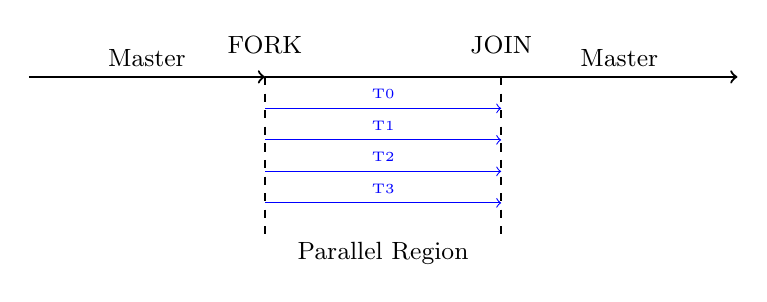
\begin{tikzpicture}[x=1.5cm,y=0.8cm]
    % Master thread line
    \draw[thick,->] (0,0) -- (2,0) node[midway,above]{\small Master};
    \draw[thick]    (2,0) -- (4,0);
    \draw[thick,->] (4,0) -- (6,0) node[midway,above]{\small Master};
    % Fork/Join markers
    \draw[thick,dashed] (2,0) -- (2,-2.5);
    \draw[thick,dashed] (4,0) -- (4,-2.5);
    \node at (2,0.5) {\small FORK};
    \node at (4,0.5) {\small JOIN};
    % Thread lines
    \foreach \y/\lbl in {-0.5/T0,-1.0/T1,-1.5/T2,-2.0/T3} {
        \draw[blue,->] (2,\y) -- (4,\y) node[midway,above,font=\tiny]{\lbl};
    }
    % Labels
    \node[font=\small] at (3,-2.8) {Parallel Region};
\end{tikzpicture}
\end{center}

\begin{enumerate}
    \item The \textbf{master thread} runs sequentially until it hits a
          \texttt{\#pragma omp parallel} block.
    \item It \textbf{forks} a team of worker threads.  All threads share the
          same address space (the same arrays in RAM).
    \item All threads execute the parallel region concurrently.
    \item At the closing brace, all threads \textbf{join} back into one.
    \item Execution continues serially until the next parallel region.
\end{enumerate}

\subsection{The Shared Memory Model}

All threads share the same physical RAM.  They can read and write the same
arrays without any explicit send/receive operations:

\begin{center}
\begin{tabular}{ccc}
Thread 0 & \multirow{4}{*}{$\longrightarrow$\quad Shared:} &
  \texttt{ratings[]}, \texttt{user\_mean[]} \\
Thread 1 & & \texttt{sim\_matrix[]}, \texttt{predictions[]} \\
Thread 2 & & (all allocated once, visible to all) \\
Thread 3 & & \\
\end{tabular}
\end{center}

\textbf{The danger}: if two threads \emph{write} to the same location at the
same time, the result is undefined — this is called a \textbf{data race}.  Our
design avoids data races by ensuring each thread writes to a \emph{disjoint}
set of indices.

% =============================================================================
\section{Key OpenMP Directives Used in Our Project}
% =============================================================================

\subsection{\texttt{\#pragma omp parallel for schedule(static)}}

\textbf{Used in:} Phase 2 (user means).

\begin{lstlisting}
#pragma omp parallel for schedule(static)
for (int u = 0; u < N_USERS; u++) {
    double sum = 0.0;  /* private -- declared inside loop body */
    int    cnt = 0;    /* private -- each thread has its own copy */
    for (int i = 0; i < N_ITEMS; i++) {
        if (R(u, i) != 0.0f) { sum += R(u, i); cnt++; }
    }
    user_mean[u] = (cnt > 0) ? (float)(sum / cnt) : 3.0f;
}
\end{lstlisting}

\textbf{Breaking it down:}

\begin{center}
\begin{tabular}{lp{9cm}}
\toprule
Clause & Meaning \\
\midrule
\texttt{parallel} & Fork a team of $T$ threads \\
\texttt{for} & Distribute loop iterations across the threads \\
\texttt{schedule(static)} & Pre-assign equal-size contiguous chunks to each
  thread at compile time.  Thread 0 gets $u \in [0, N/T)$, Thread 1 gets
  $[N/T, 2N/T)$, etc. \\
\bottomrule
\end{tabular}
\end{center}

\textbf{Why \texttt{static} here?}  Every user row involves exactly the same
work: scan \texttt{N\_ITEMS} items.  Equal work per iteration $\Rightarrow$
static scheduling gives perfect load balance with zero runtime overhead.

\textbf{Race safety:}  Thread $t$ only writes \texttt{user\_mean[u]} for its
assigned $u$ values.  No two threads share an index.  Variables \texttt{sum}
and \texttt{cnt} are declared inside the loop body and are therefore
automatically \emph{thread-private} in OpenMP.

\subsection{\texttt{\#pragma omp parallel for schedule(dynamic, 4)}}

\textbf{Used in:} Phase 3 (similarity matrix).

\begin{lstlisting}
#pragma omp parallel for schedule(dynamic, 4)
for (int u = 0; u < N_USERS; u++) {
    for (int v = u + 1; v < N_USERS; v++) {
        float s = pearson_similarity(u, v);
        SIM(u, v) = s;
        SIM(v, u) = s;  /* mirror -- race-free (see analysis below) */
    }
}
\end{lstlisting}

\textbf{Why \texttt{dynamic} here?}

The inner loop runs $N_{\text{USERS}} - u - 1$ times.  Outer iteration $u=0$
does $999$ Pearson calls; $u=999$ does $0$.  Work \emph{decreases} with $u$.
Static scheduling would give Thread 0 (small $u$) far more work than Thread 3
(large $u$) — severe load imbalance.

Dynamic scheduling uses a work queue: whenever a thread finishes its current
chunk of 4 iterations, it pulls the next 4 from the queue.  Fast-finishing
threads pick up more work, keeping all cores busy.

\textbf{Race-free write proof:}  Thread $t$ owns outer iterations in some set
$U_t$.  For each $u \in U_t$, it writes \texttt{SIM(u,v)} for all $v > u$,
and \texttt{SIM(v,u)} for the same $v$.  Could two threads write to the same
cell?  Thread $A$ (owns $u=5$) writes \texttt{SIM(7,5)}.  Thread $B$ (owns
$u=7$) writes \texttt{SIM(7,v)} only for $v > 7$, i.e. $v \geq 8$.  So
Thread $B$ never writes \texttt{SIM(7,5)}.  All writes are disjoint
$\Rightarrow$ no race.

\subsection{\texttt{\#pragma omp parallel} + Thread-Private Buffer}

\textbf{Used in:} Phase 4 (predictions).

\begin{lstlisting}
#pragma omp parallel           /* fork T threads */
{
    /* malloc() is thread-safe: each call returns a DIFFERENT allocation */
    SimPair *nbrs = (SimPair *)malloc(N_USERS * sizeof(SimPair));

    #pragma omp for schedule(dynamic, 2)
    for (int u = 0; u < N_USERS; u++) {
        /* ... use nbrs (private to this thread) ... */
    }
    /* implicit barrier: all threads done with the for loop */

    free(nbrs);   /* each thread frees its own buffer */
}
/* threads join here */
\end{lstlisting}

\textbf{Why not \texttt{\#pragma omp parallel for}?}  That single directive
would fork and immediately distribute the loop.  We need each thread to first
allocate its own \texttt{nbrs} buffer \emph{before} the loop starts.  Using
\texttt{\#pragma omp parallel} (fork only), then \texttt{\#pragma omp for}
(distribute) inside the block achieves this.

\subsection{\texttt{reduction(+:err)}}

\textbf{Used in:} Phase 5 (MAE evaluation).

\begin{lstlisting}
double err = 0.0;
#pragma omp parallel for reduction(+:err) schedule(static)
for (int t = 0; t < test_size; t++)
    err += fabs(PRED(...) - test_set[t].rating);
/* After this: err = sum across all test entries */
\end{lstlisting}

\textbf{What \texttt{reduction} does:}
\begin{enumerate}
    \item Gives each thread a \emph{private copy} of \texttt{err}, initialised
          to the identity element (0 for \texttt{+}).
    \item Each thread accumulates into its own private copy — no locks needed.
    \item At the end of the parallel region, OpenMP \emph{combines} all private
          copies using the specified operator (\texttt{+}) into the original
          shared variable.
\end{enumerate}

\textbf{Why not use \texttt{\#pragma omp atomic}?}  An atomic update would
\emph{serialise} every addition — threads must queue up one at a time.
Reduction is parallel all the way; the final merge is $O(T)$ additions, negligible.

% =============================================================================
\section{OpenMP Variables: Shared vs. Private}
% =============================================================================

By default in OpenMP:
\begin{itemize}
    \item Variables declared \emph{outside} the parallel region are
          \textbf{shared} — one copy, visible to all threads.
    \item Variables declared \emph{inside} the parallel region are
          \textbf{private} — one copy per thread, independent.
\end{itemize}

\begin{center}
\begin{tabular}{lll}
\toprule
Variable & Type & Reason \\
\midrule
\texttt{ratings[]} & Shared & Read-only after Phase 1; no race \\
\texttt{user\_mean[]} & Shared & Each thread writes to disjoint indices \\
\texttt{sim\_matrix[]} & Shared & Disjoint write indices \\
\texttt{predictions[]} & Shared & Disjoint write indices \\
\texttt{sum, cnt} (Phase 2) & Private & Declared inside loop body \\
\texttt{nbrs[]} (Phase 4) & Private & \texttt{malloc}ed inside parallel block \\
\texttt{err} (Phase 5) & Reduction & Explicitly listed in \texttt{reduction} clause \\
\bottomrule
\end{tabular}
\end{center}

% =============================================================================
\section{Timing with OpenMP}
% =============================================================================

\begin{lstlisting}
#include <omp.h>
static inline double now_sec(void) { return omp_get_wtime(); }
\end{lstlisting}

\textbf{Why \texttt{omp\_get\_wtime()} not \texttt{clock()}?}

\texttt{clock()} returns total \emph{CPU time} summed across all threads.  If
4 threads each work for 1 second, \texttt{clock()} reports 4~seconds.
\texttt{omp\_get\_wtime()} returns \emph{wall-clock elapsed time} — 1 second
in this case.  We need wall-clock time to compute speedup correctly.

% =============================================================================
\section{Implicit Barriers in OpenMP}
% =============================================================================

OpenMP inserts an \textbf{implicit barrier} (all threads wait) at:
\begin{itemize}
    \item The end of a \texttt{\#pragma omp for} block
    \item The end of a \texttt{\#pragma omp parallel} block
    \item The end of a \texttt{\#pragma omp single} or \texttt{sections} block
\end{itemize}

These barriers ensure that all threads have completed Phase $n$ before
any thread starts Phase $n+1$.  In our code, the function returns only after
all threads have joined, so phases are naturally ordered.

% =============================================================================
\section{Schedule Comparison}
% =============================================================================

\begin{center}
\begin{tabular}{llll}
\toprule
Schedule & How chunks assigned & Best when & Overhead \\
\midrule
\texttt{static} & Fixed at compile time & Equal work/iteration & None \\
\texttt{dynamic,C} & On-demand, chunk $C$ & Unequal work/iteration & Queue lookup \\
\texttt{guided} & Decreasing chunk sizes & Irregular work & Moderate \\
\bottomrule
\end{tabular}
\end{center}

In our project:
\begin{itemize}
    \item Phase 2 (means): \texttt{static} — every row scans exactly
          \texttt{N\_ITEMS} items.
    \item Phase 3 (similarity): \texttt{dynamic,4} — inner loop size
          decreases from $N-1$ to $0$ as $u$ increases.
    \item Phase 4 (predictions): \texttt{dynamic,2} — item density varies
          across users.
\end{itemize}

% =============================================================================
\section{What Changed from Serial to OpenMP}
% =============================================================================

The data structures, algorithm, and output are \textbf{identical}.  The only
changes are:

\begin{enumerate}
    \item Add \texttt{\#include <omp.h>}
    \item Replace \texttt{now\_sec()} body with \texttt{omp\_get\_wtime()}
    \item Add \texttt{\#pragma omp parallel for schedule(static)} before
          Phase 2 loop
    \item Add \texttt{\#pragma omp parallel for schedule(dynamic, 4)} before
          Phase 3 loop
    \item Wrap Phase 4 in \texttt{\#pragma omp parallel} with thread-private
          \texttt{nbrs} allocation
    \item Add \texttt{reduction(+:err)} to Phase 5
    \item Compile with \texttt{-fopenmp}; run with
          \texttt{OMP\_NUM\_THREADS=4}
\end{enumerate}

This demonstrates one of OpenMP's key strengths: \textbf{incremental
parallelisation} — you can add parallelism to a serial program with minimal
structural changes.

% =============================================================================
\section{Compile and Run}
% =============================================================================

\begin{verbatim}
# Compile (add -fopenmp to activate OpenMP support)
gcc -O2 -Wall -fopenmp -o openmp_rec openmp/openmp_recommender.c -lm

# Run with different thread counts
OMP_NUM_THREADS=1  ./openmp_rec 1000 1000   # serial-equivalent
OMP_NUM_THREADS=2  ./openmp_rec 1000 1000
OMP_NUM_THREADS=4  ./openmp_rec 1000 1000
OMP_NUM_THREADS=8  ./openmp_rec 1000 1000
\end{verbatim}

\textbf{Without \texttt{-fopenmp}}: all \texttt{\#pragma omp} lines are
silently ignored; the program runs serially.  Useful for debugging: compile
without the flag and verify the output matches the serial baseline exactly.

% =============================================================================
\section{Key Points to Explain in a Presentation}
% =============================================================================

\begin{enumerate}
    \item \textbf{Why not parallelise Phase 1 (data generation)?}  C's
          \texttt{rand()} is not thread-safe — calling it from multiple threads
          simultaneously causes a data race on its internal state.  Different
          random sequences would mean different data, so the MAE comparison
          would be meaningless.
    \item \textbf{How do we know there are no race conditions?}  Each thread
          writes to a unique range of row indices.  We verified this by
          checking the \texttt{[Check]} sim-matrix checksum matches the serial
          baseline exactly.
    \item \textbf{Why does efficiency drop with more threads?}  Serial
          fractions (Phase 1, output), synchronisation overhead at barriers,
          and cache coherence traffic between cores all limit efficiency.
    \item \textbf{What is the maximum speedup for our workload?}  Phase 1
          is serial.  If Phase 1 takes $\sim$1\% of total time, Amdahl's Law
          gives $S_{\max} \approx 100\times$ — but in practice cache effects
          and overhead limit it to $6$--$7\times$ on 8 cores.
\end{enumerate}

\vfill
\begin{center}
    \small\textit{Group 11 — EC7207 High Performance Computing}
\end{center}

\end{document}
